\documentclass[11pt]{article}
\usepackage{graphicx}
\usepackage{amssymb}
\usepackage{epstopdf}
\usepackage{natbib}
\usepackage[pdftex]{graphicx}
\DeclareGraphicsExtensions{.png,.pdf}
\graphicspath{{images/}}

\textwidth = 6.5 in
\textheight = 9 in
\oddsidemargin = 0.0 in
\evensidemargin = 0.0 in
\topmargin = 0.0 in
\headheight = 0.0 in
\headsep = 0.0 in
\parskip = 0.0in
\parindent = 0.1in

\renewcommand{\textfraction} {0}
\renewcommand{\bottomfraction} {1}
\renewcommand{\topfraction} {1}
\renewcommand{\floatpagefraction} {1}


\renewcommand{\labelenumi}{(\alph{enumi})}

\newtheorem{theorem}{Theorem}
\newtheorem{corollary}[theorem]{Corollary}
\newtheorem{definition}{Definition}

\title{Letter-Value Box Plots: 
Adjusting Box Plots for Large Data Sets}
\author{Heike Hofmann, Karen Kafadar, Hadley Wickham}

\begin{document}
\maketitle

\subsection*{Abstract}

Conventional boxplots (Tukey 1977) are useful
displays for conveying rough information about the
central 50\% of the data and the extent of the data.
For moderate-sized data sets ($n < 1000$), detailed 
estimates of tail behavior beyond the quartiles may 
not be trustworthy, so the information provided by 
boxplots is appropriately somewhat vague beyond 
the quartiles,
% with only a ``whisker'' that shows the distance 
% between the quartile and the ``adjacent value'' 
% (value of the observation just inside the inner fence). 
and the expected number of ``outliers'' and ``far-out'' 
values for a Gaussian sample of size $n$ is often
less than 10 (Hoaglin, Iglewicz, and Tukey 1986).
Large data sets ($n \approx 10,000-100,000$)
afford more precise estimates of quantiles in the
tails beyond the quartiles and also can be expected
to present a large number of ``outliers'' (about
0.4 + 0.007$n$).  The letter-value box plot addresses
both these shortcomings:  it conveys more detailed 
information in the tails using letter values, only
out to the depths where the letter values are reliable
estimates of their corresponding quantiles 
(corresponding to tail areas of roughly $2^{-i}$);
``outliers'' are defined as a function of the most extreme
letter value shown.  All aspects shown on the
letter-value boxplot are actual observations, thus
remaining faithful to the principles that governed
Tukey's original boxplot.  We illustrate the 
letter-value boxplot with some actual examples that
demonstrate their usefulness, particularly for
large data sets.

\textit{Key words}: boxplots, quantiles, letter value display, 
fourth, order statistic, tail area

\section{Introduction}

Since  \citet{tukey72} introduced box plots, various modifications 
to them have been proposed.  
Tukey himself changed the definition of whisker length,
from  ``quartiles to extremes'' in 1972
to  ``quartiles to adjacent values'' \citep{eda},
the standard commonly accepted today.
McGill, Tukey, and Larsen (1978) enhanced box plots with 
variable widths (widths proportional to square root of 
the sample sizes) and notches (half-lengths of approximate 
intervals for comparing medians). Subsequent enhancements
include vase plots \citep{vase}, violin plots \citep{violin}, 
and box-percentile plots \citep{box.percentiles}.
These later proposals attempt to display more detailed
notions of the distributions of the data, through the use
of nonparametric density estimates.  The added detail is
especially useful for larger sample sizes, but these later 
displays depend on the specific estimation procedure.  
Benjamini (1988) acknowledged this dependence, in connection 
with his proposed vase plots, on the method of estimation
(kernel density estimate, nearest-neighbor, spline, etc.)
as well as on a bandwidth or other smoothing parameter; 
hence the same data can give rise to different displays
depending on the estimate.  In contrast, the boxplot in  
its original form displayed only actual observations 
(median, fourths, adjacent values, outliers).  
Larger sample sizes also tend to result in more extreme
values, some of which might be presumed to be outliers.
The conventional boxplot (Tukey 1977; Emerson and Strenio
1983) labels an observation as ``outside'' if it lies 
outside the ``inner fences'' defined by the pair of 
numbers $[L_F - k(U_F - L_F), U_F + k(U_F - L_F)]$ 
where $L_F$ and $U_F$ denote the lower and upper
fourths, respectively (estimates of the lower and
upper population quartiles) and $k = 1.5$ (Tukey 1972 
actually had a different definition);
in a Gaussian sample of size $n$,
the expected number of labeled ``outliers'' grows 
approximately linearly with $n$, roughly
0.4 + 0.007$n$ (approximation due to Hoaglin, Iglewicz, 
and Tukey 1986), a very large number when $n$ is large.  
Hoaglin and Iglewicz (1987) calculated values of $k$ to 
maintain the expected rate of labeled ``outliers'' at 5\% 
or 10\% for values of $n$ from 5 to 300 and found that
$k = 2.2-2.4$ for an outside rate of 5\% when the
fourths are defined as those order statistics that
have depth $n/4 + 5/12$.  Even with an increased $k$
to ensure a fixed outside rate of 5\%, however, 
boxplots constructed from samples of 100,000 or more
can be expected to label 5000 observations, far too
many for detailed inquiry.

The conventional box plot is therefore very useful for 
small or moderate-sized data sets, but somewhat inadequate
for very large data sets, in two ways.  First, while 
estimates of quantiles in the tails of a distribution 
beyond the quartiles may be imprecise for smaller data sets
(and thus probably better not shown), large data sets 
afford somewhat more reliable estimates of tail behavior.  
Second, because the expected outside
rate goes to 1 for fixed $k$ as $n$ gets large, 
the conventional boxplot can be expected to label
increasing numbers of observations as ``outliers''.
The letter value box plot that we propose
addresses both of these shortcomings for large data sets.
In addition, its construction resembles the original 
boxplot by displaying only actual values that occur in 
the sample.  The rules for constructing the letter value
box plot reduce to the conventional box plot for small
data sets.

Conventional boxplots rely on quartiles for the boxes to ensure 
``relative insensitivity of summaries and subsequent calculations 
to unusual observations.'' (citation for this quotation?)  
Hence, the breakdown point of default box plots is 25\%; 
i.e., only if 25\% of all data points or more are affected 
will the summary statistics and outlier identification change.
This high breakdown is one of the valuable features of boxplots.  
Moreover, the relatively low uncertainty in the fourths as 
estimates of the quartiles argues in favor of using the fourths 
in the rule for labeling ``outliers'': 
the standard deviation of the fourths equals roughly 
$\sqrt{\frac{1}{4} \cdot \frac{3}{4} / n} / \phi(\frac{1}{4})$
= $1.12 / \sqrt{n}$ for a standard Gaussian distribution with
probability density function $\phi(\cdot)$, or a 2-SD uncertainty
of roughly 0.22$\sigma$ for Gaussian samples of size 100 (reference).
Estimates of the population quantiles in the tails of a distribution
based on order statistics are rather variable.  For small samples,
then restricting attention to only estimates of the population
median and quartiles, with some broad indication of the tail length
beyond the quartiles, is likely to be about all that the data can
support.  The situation is quite different for large sample sizes.
Estimates with quantiles corresponding to smaller tail areas are
more reliable and outliers need to be kept to a managable number.
Displays of large data sets can afford to indicate more confidently
estimates of quantiles in the tails.  Hence, an alternative
rule for of labeling outliers in large samples may be based
on a function of a fixed number of observations
beyond the last quantile which can be estimated reliably.


\begin{figure*}[hbt]
\begin{center}
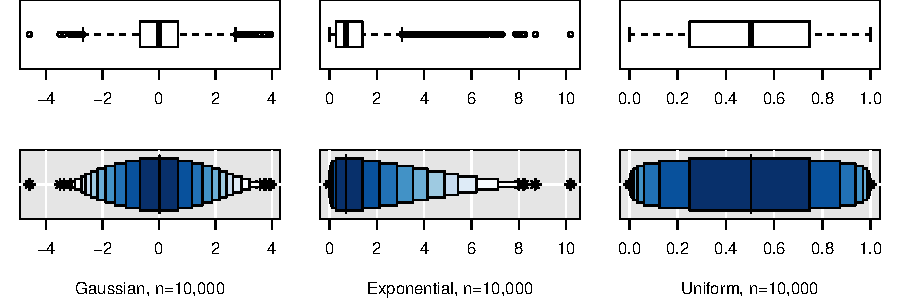
\includegraphics[width=6in]{boxplots.pdf}
\caption{\it \label{stackbox} Letter-Value Box Plots and standard 
box plots for data from three different distribution.  Each plot 
shows 10,000 data points.  From top to bottom samples come from 
(a) $N(0,1)$, (b) $Exp_1$, and (c) $U[0,1]$. }
\end{center}
\end{figure*}


It is instructive to recall the location of the displayed
values for given theoretical populations.
For a standard Gaussian whose observations are i.i.d.,
the theoretical fourths can be expected to appear at 
$\pm  0.6745$, yielding an interquartile range 
(estimated by the fourth-spread) of 1.3490.
Theoretical whiskers therefore lie at 
$\pm (0.6745 + 1.5 \cdot 1.3490) = \pm 2.6980$.  
The area of box and whiskers covers more than 99.3\% of the 
distribution --- leaving about 0.7\% of the points as outliers 
(and $2.34 \cdot 10^{-04}$\% ``far outliers'') -- hence the
approximation in Hoaglin, Iglewicz, and Tukey 1986 for the
expected number of labeled outliers (0.4 + 0.007$n$).
In the setting of an exponential distribution with unit mean, 
the theoretical hinges lie at 0.2877 and 1.3863, so the fourth
spread will be roughly 1.0986.  The box and whiskers therefore
cover an area of roughly 0.9519, leading to an outside rate
of almost 5\% and a ``far-out'' rate of almost 1\%.

Here, we follow the approach of Hoaglin and Iglewicz (1987)
by allowing our displays to label outliers in terms
of fixed counts (or, given the sample size, a fixed outside rate),
again based on the fourths, which avoids the dependence of the
outside rate for any particular batch of numbers on its
underlying distribution.
The quantiles that we use for both the display and the outlier
rule are the letter values (Hoaglin, 1983), which extend the
notion of median and fourths in a natural way.

\section {Letter values}

Let $X_{(1)}$, ...  $X_{(n)}$ denote the order statistics
from a sample of size $n$.
The letter values are those order statistics having specific
depths, defined recursively starting with the median.
The depth of the median, $d_M$, of a sample of size $n$
is defined as $d_M = (1 + \lfloor n \rfloor)/2$; the depths
of successive letter values (F=fourths, E=eighths, 
D=sixteenths, C=thirty-seconds, ...) are defined recursively 
as $d_i = (1 + \lfloor d_{i-1} \rfloor)/2$.  
The $i^{th}$ lower and upper letter values ($LV_i$) are 
thus defined as $L_i = X_{(d_i)}$ and
$U_i = X_{(n-d_i+1)}$.
(If the depth involes a ``half'' then the lower letter 
value is defined as the average of the two adjacent order
statistics, $X_{\lfloor d_i \rfloor}$ and
$X_{\lceil d_i \rceil}$, and similarly for the upper
letter value.)
The advantage of this definition for the letter values
is that the median of this sample quantile from a
continuous distribution $F(\cdot)$ is very close to
$F^{-1} ((i - \frac{1}{3})/(n + \frac{1}{3})$, for a 
wide range of $F$, $n$, and $i$ (Hoaglin 1983).
Because each depth is roughly half of the previous depth,
the letter values approximate the quantiles corresponding
to tail areas $2^{-i}$.
The letter value display for the 1980 populations
and the log populations
of the 3068 counties in the continential United States
(plus the District of Columbia) is shown in Table 1.
Along with the letter values are shown the midspreads
(average of the upper and lower letter values), the
spread between the letter values, and ``pseudo-sigma''
(Hoaglin 1983, p.40), the sample letter-value spread 
divided by the theoretical
letter-value spread for a standard Gaussian
density (e.g., pseudo-sigma based on the fourths is 
the fourth spread divided by 1.3490).
For a nicely symmetric population, the midspreads should
be constant, and, for a distribution with Gaussian-like
tails, the pseudo-sigmas should also be fairly stable.
Both the midspreads and the pseudo-sigmas are much more
nearly constant for the log populations than for the
untransformed populations.


\begin{verbatim}
                  Table 1

           Letter value display for 1980
         populations in 3068 U.S. counties

    Depth  Lower   Upper      Mid  Spread   pseudo-s
M  1534.5  218.0   218.0   218.00     0.0     0.0000
F   767.5  105.0   511.0   308.00   406.0   601.9365
E   384.0   65.0  1082.0   573.50  1017.0   884.0792
D   192.5   39.0  2280.0  1159.50  2241.0  1460.7718
C    96.5   25.0  4572.0  2298.50  4547.0  2441.0384
B    48.5   17.5  6641.5  3329.50  6624.0  3075.3878
A    24.5   10.5  9694.5  4852.50  9684.0  4005.6933
Z    12.5    8.0 14742.5  7375.25 14734.5  5539.1452
Y     6.5    6.5 18972.5  9489.50 18966.0  6572.5570
X     3.5    4.5 38316.0 19160.25 38311.5 12369.4452
W     2.0    4.0 70716.0 35360.00 70712.0 21446.1187
V     1.5    2.5 72745.5 36374.00 72743.0 20860.5759
U     1.0    1.0 74775.0 37388.00 74774.0 20383.6663

             Letter value display for 1980
         log populations in 3068 U.S. counties

    Depth  Lower   Upper      Mid  Spread   pseudo-s
M  1534.5 2.3385  2.3385   2.3385  0.0000     0.0000
F   767.5 2.0212  2.7084   2.3648  0.6872     1.0189
E   384.0 1.8129  3.0342   2.4236  1.2213     1.0617
D   192.5 1.5911  3.3579   2.4745  1.7669     1.1517
C    96.5 1.3979  3.6601   2.5290  2.2622     1.2144
B    48.5 1.2429  3.8223   2.5326  2.5794     1.1976
A    24.5 1.0207  3.9865   2.5036  2.9658     1.2268
Z    12.5 0.9031  4.1685   2.5358  3.2654     1.2276
Y     6.5 0.8116  4.2780   2.5448  3.4664     1.2013
X     3.5 0.6505  4.5512   2.6009  3.9007     1.2594
W     2.0 0.6021  4.8495   2.7258  4.2475     1.2882
V     1.5 0.3010  4.8616   2.5813  4.5606     1.3078
U     1.0 0.0000  4.8738   2.4369  4.8738     1.3286


\end{verbatim}

\section{Letter value box plots}

Letter-Value Box Plots are based on these letter-value statistics: 
with one box for each pair of lower and upper letter-values.
The median is shown by a vertical line segment (or an asterisk),
and the innermost box is drawn at the lower and upper fourths, 
as in the conventional boxplot.
A slightly narrower box is drawn between at the lower
and upper eighths, and narrower one still at the lower
and upper sixteenths.
We continue in this fashion until we reach a stopping
rule that depends on the sample size; beyond the
most extreme box, all points beyond these limits are
identified as individual points.
In practice, the software for creating this display
proceeds from the outermost box to the innermost (``fourths'')
box, so the innermost boxes are shaded more heavily,
indicating a higher data density.
Boxes with matching heights correspond to the same depths.
With this definition, the expected proportion of the 
sample beyond the end of a box (roughly $1/2^i$)
equals the expected proportion between this end 
and the end of the next bigger box
(i.e., roughly $1/2^{i-1} - 1/2^i$ = $(1/2^{i-1})(1 - \frac{1}{2})$
= $1 / 2^i$).
For samples of size $n$ the lower and upper $i$th letter statistics 
are minimum and maximum, respectively, for all $i$ with $2^i \ge n$. 

Letter value boxplots for three different distributions are 
shown in Figure \ref{stackbox}. 
Each panel in Figure \ref{stackbox} displays a sample of 10,000 
data points (top = standard Gaussian, middle = exponential 
with mean 1, bottom = standard uniform),
first using the proposed letter value boxplot
up to letter Y, corresponding roughly to tail area $2^{-9}$
= 1/512 (left side), and then with the
the conventional boxplot (right side).
Comparing the top (Gaussian) and bottom (Uniform) letter
value displays, overall darker displays correspond to distributions 
with lighter tails.  This is shown more forcefully in
Figure \ref{t-dist} with two extreme examples for heavy tail 
distributions: 10,000 samples from a $t$ distribution with 2 
degrees of freedom (top rows) and with 3 degrees of freedom 
(bottom rows), again with both the letter value boxplot and
with the standard boxplot. (Can we put on same scale?)

\begin{figure*}[hbt]
\begin{center}
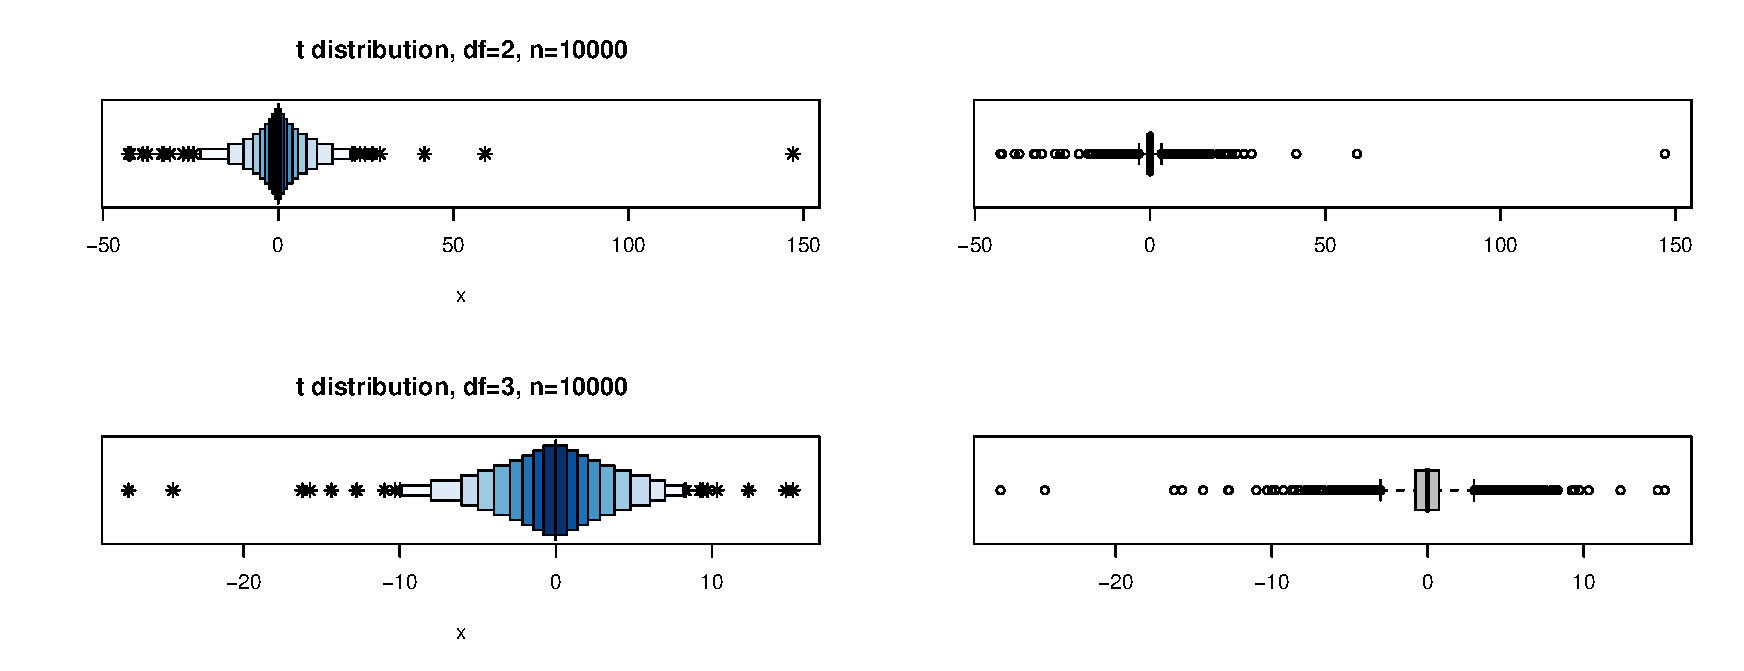
\includegraphics[width=6in]{t-distribution.pdf}
\caption{\it \label{t-dist} Letter-Value boxplots and standard boxplots 
for samples of two $t$ distributions. The two top plots 
show $X \sim t_2$, the two lower plots show $X \sim t_3$. }
\end{center}
\end{figure*}

Figure \ref{lvpops} shows the letter value boxplots
and the conventional boxplots for the data in Table 1,
corresponding to the 1980 populations and log populations
of the 3068 counties in the United States.  While the
skewness in the distribution of the populations is
clear from both the letter-value boxplot and the
conventional boxplot, the former shows more clearly
that the right tail of the log populations above the 
median is somewhat more extended than the left tail
below the median (i.e., the boxes to the right of
the median are slighly longer than those to the
left of the median).


\begin{figure*}[hbt]
\begin{center}
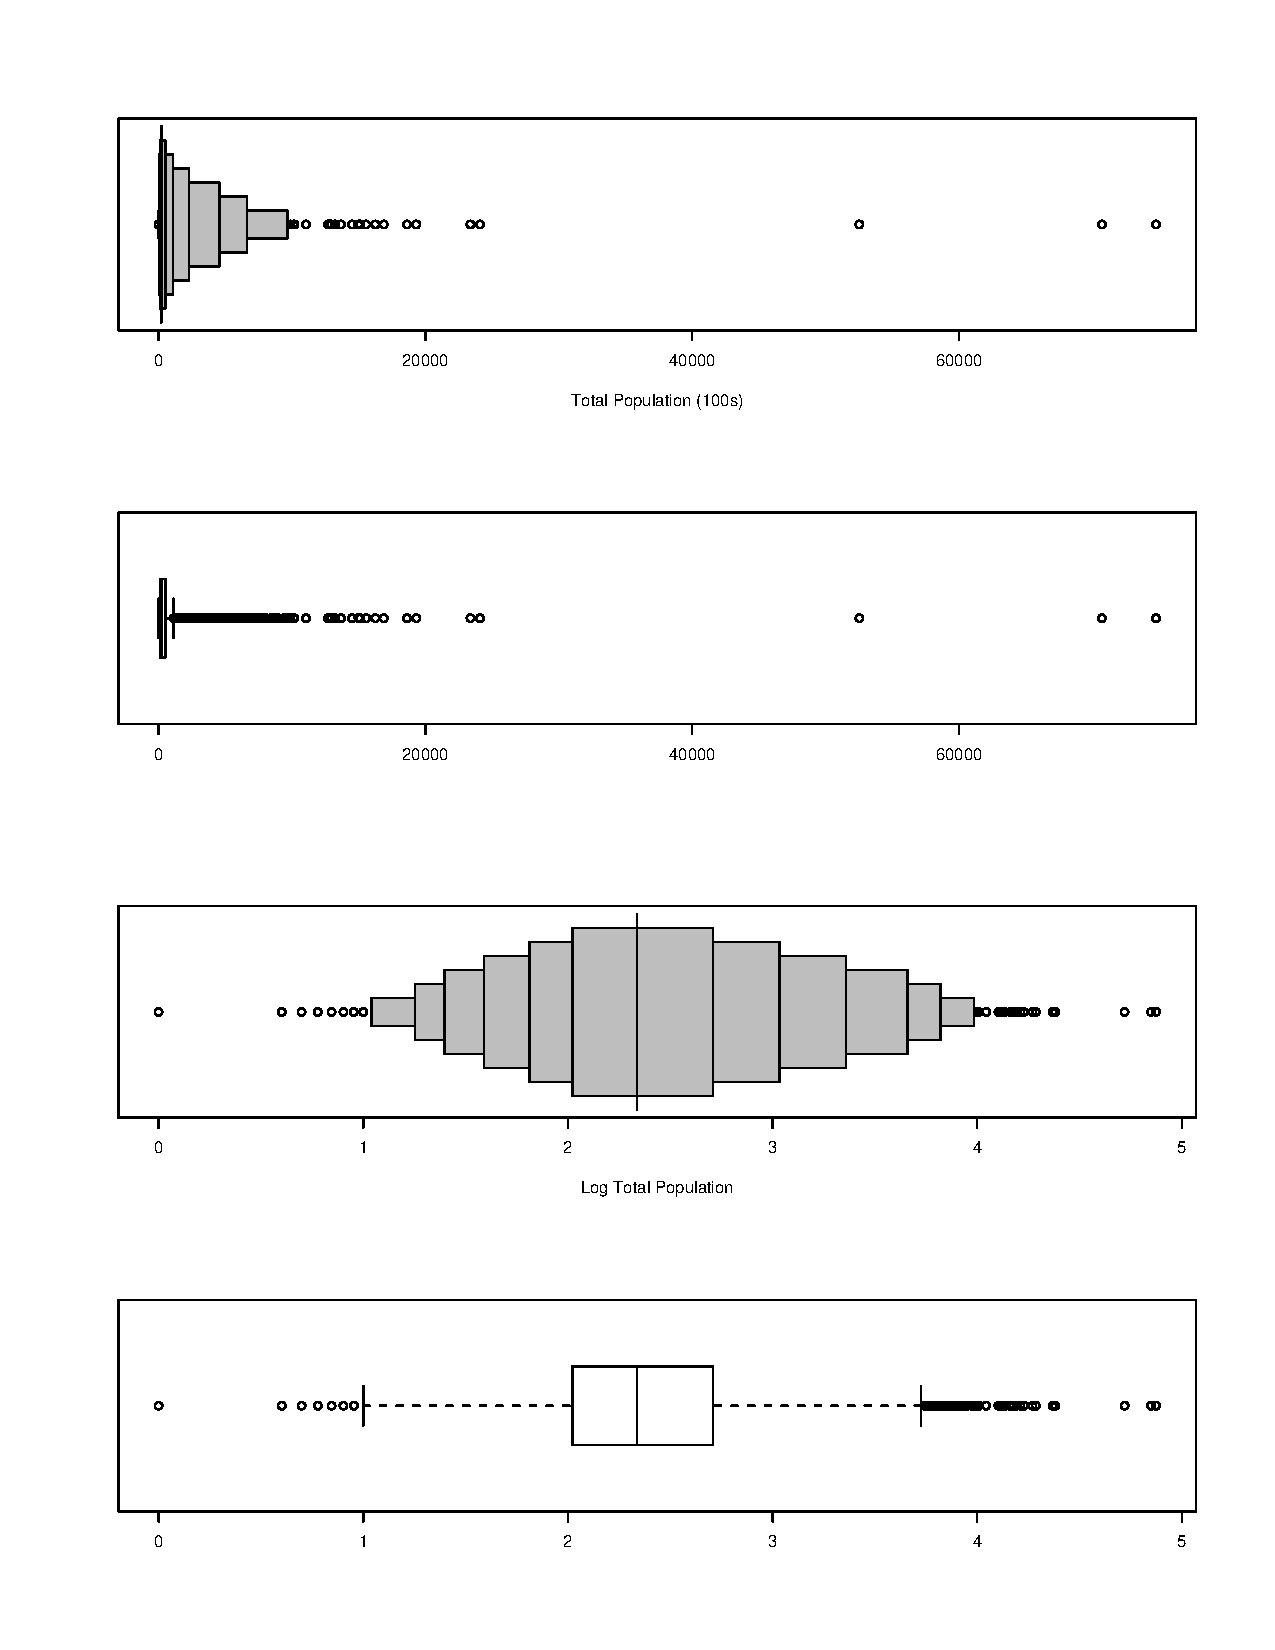
\includegraphics[width=6in]{lvplot.pdf}
\caption{\it \label{lvpops} Letter-Value Box Plots and standard 
box plots for the 1980 populations and log populations of 3068
counties in the continental United States.}
\end{center}
\end{figure*}



\section{Extent of letter value boxplots}

As indicated in the introduction, a serious
drawback to the conventional boxplot for large
data sets is the tendency for an exhorbitant
number of labeled outliers.  Figure \ref{kkewbox} 
shows a boxplot of a measure of the duration of
135,000 Internet sessions, stratified
into 31 groups based on the logarithms of
the number of bytes transferred during the
session (Kafadar and Wegman 2006).
With an average of almost 4,000 points in any one category,
the number of labeled outliers is huge --- far too 
many to investigate individually.  This large number
makes it difficult to distinguish between genuine
``outliers'' (observations from a different distribution)
from long-tailed distributions.

\begin{figure*}[hbt]
\begin{center}
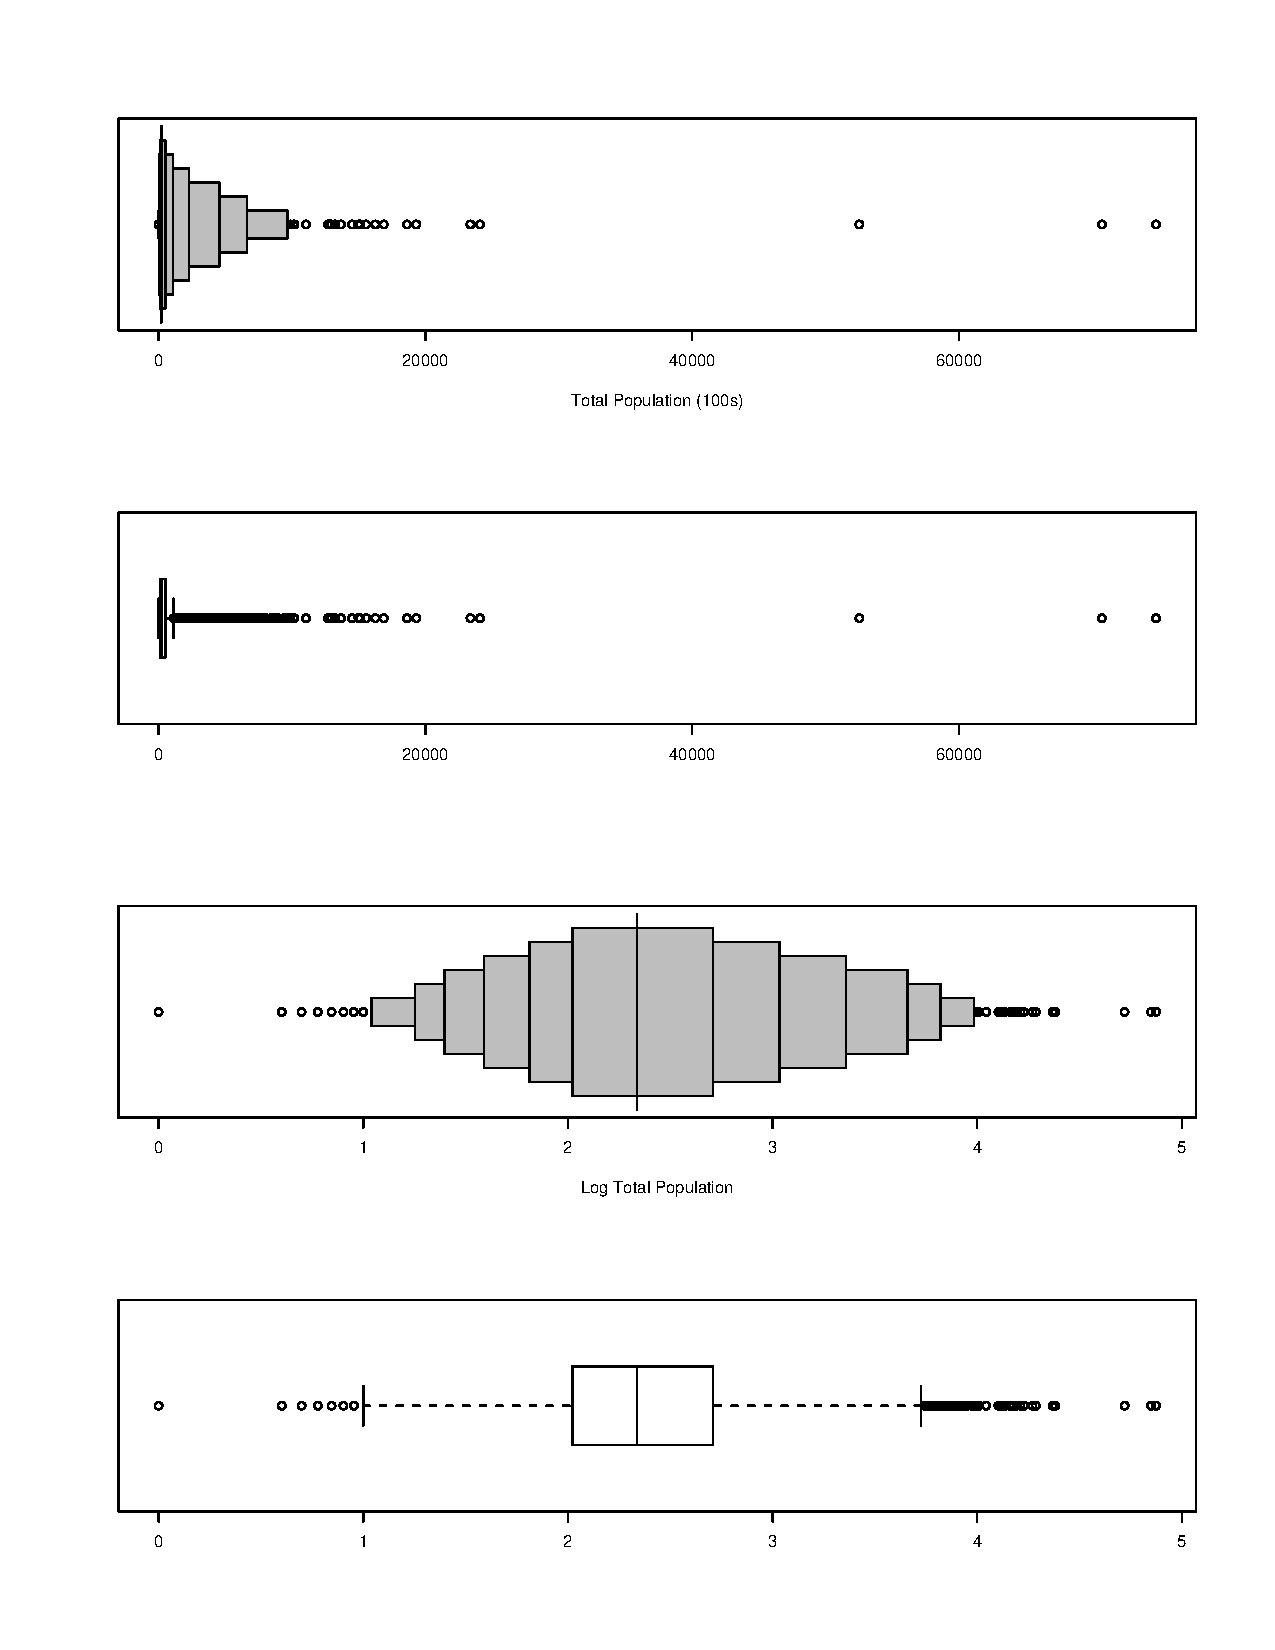
\includegraphics[width=6in]{lvplot.pdf}
\caption{\it \label{kkewbox} Box Plots of (transformed)
duration for 135,000 internet sessions, grouped by 
ranges of (transformed) byte lengths for the sessions.}
\end{center}
\end{figure*}

The standard letter value display (cf. Table 1) stops with
that letter value having depth=1 (i.e., the extremes).
In many cases, these extremes could lie far from the
rest of the sample, particularly if they are outliers.
Just as the whiskers in today's conventional boxplot 
extend to the adjacent values (observations just
inside the inner fences, which can be the extremes
in samples with no labeled outliers), the extent
of the boxes in a letter value boxplot need not
necessarily go all the way out to the extremes.
We need a rule for determining how many boxes to
show in a letter-value boxplot, which will determine
the number of labeled outliers.

In many of the displays in \textit{Exploratory
Data Analysis}, Tukey identified 5--8 extreme points.
As a rough guideline, we can choose the extent
of the letter value boxplot display so that
the last set of boxes encompasses all but
5--8 most extreme observations.
Recall that the depth of the $k^{th}$ letter value,
$d_k$, is defined in terms of the previous depth:
$d_k = (1 + \lfloor d_{k-1} \rfloor)/2$, which
implies that 
$2 d_{k-1} \leq d_{k-1} \leq 2 d_k - \frac{1}{2}$.
If we stop the letter value boxplot display at
$LV_k$ where $k = \lceil \log_2 n \rceil - 4$,
then we can expect to label 5--8 observations
in each tail.  For samples of size
10,000 as in Figure \ref{stackbox},
$k = \lfloor log_2 10000 \rfloor - 4$ = 13 -- 4 = 9,
so 9 letter values beyond the median are shown
(F, E, D, C, B, A, Z, Y, X -- i.e., down to
tail area of roughly 1/1024 $\approx$ 0.001).
For the 3068 counties, 
$k = \lfloor log_2 3068 \rfloor - 4$ = 11 -- 4 = 7,
so Figure \ref{kkewbox} shows
7 letter values (M, F, E, D, C, B, A).


An alternative criterion fixes the number of
labeled outliers in terms of a percentage of
the overall sample size.  Letting $p$ denote
this proportion, the last set of boxes to be
drawn ends with depths
\begin{center}
$k = \lceil \log_2 n \rceil - \lceil \log_2 (np) \rceil + 1$
\end{center}
This criterion results in the same rule 
as the previous rule for the samples in
Figure \ref{stackbox} ($n = 10,000$) when 
$p$ lies between 0.004 and 0.006 (0.4\% -- 0.6\%), 
and in Figure \ref{lvpops} ($n = 3068$) when
$p$ lies between 0.011 and 0.020 (1.1\% -- 2.0\%).

% A third approach is to base the final $k$ on 
% the ``trustworthiness'' of the $k^{th}$ letter value 
% as an estimate of the corresponding population quantile.
% 
% Let us assume, that the $k$th letter-value statistic is the 
% minimal letter-value statistic with depth 1, i.e. $d_k = 1$. 
% This implies  $d_{k-1} = 1.5$ (the median of two observations). 
% For $d_{k-2}$ we have a minimum of 2 and a maximum of 2.5, 
% based on at least 3 observations and at most 4. From this, 
% the $k-3$ letter-value statistics has a depth of at least 3 
% and at most 4.5. $d_{k-4}$ is at least 5 and at most 8.5, 
% $d_{k-5}$ is at least 9 and at most 16.5.
% For $d_{k} \ge 1.5$ the general rule holds, that 
% $2d_{k} - 1 \le d_{k-1} \le 2d_{k} -0.5$. 
% 
% Based on these considerations, we can now try to come up with 
% a default percentage or default number of points, which we 
% want to draw and identify individually. This will also determine 
% the number of  boxes we have to draw.
% 
% In almost all of his publications, Tukey made sure to identify 
% and label the five most extreme points in a boxplot at each end 
% of the scale. We could use this value as a guideline and show 
% five to eight points individually. For $n$ observations, 
% using $k$ letter-value statistics with $k$ given as
% \[
% k = \lceil \log_2 (n) \rceil - 4,
% \]
% ensures between 5 and 8 individual points on each side. 
% 
% Another alternative is, to fix the number of individually drawn 
% points in terms of a percentage of the overall sample size. 
% Assuming, we want to have $p$ percent points marked as outliers, 
% we will use $k$ letter-value statistics with $k$:
% \[
% k = \lceil \log_2 (n) \rceil - \lceil \log_2 (0.01 n p) \rceil + 1.
% \]

A third approach is to base the final $k$ on the ``trustworthness'' 
of the $k^{th}$ letter value as an estimate of the corresponding
population quantile. 
``Trustworthiness'' here will be characterized by the extent of an
an approximate 95\% confidence interval around a given letter value;
if it overlaps that for the subsequent letter value, then the
uncertainty for the given letter value is high enough that we
will not display it.  Thus, boxes are shown for those
letter values whose approximate 95\% confidence intervals
exclude the neighboring letter values. 
Since letter values can be viewed as medians between the
extreme the previous letter value,
a simple rule of thumb for an approximate 
$1-\alpha$ confidence interval for the median of $n$ values 
(with $n > 10$) has $0.5 \sqrt{n} z_{1-\alpha/2}$ observations 
on both sides of the sample median and rounding out to the next integer, 
where $z_{1-\alpha/2}$ is the ${1-\alpha/2}$ quantile of a standard 
Gaussian distribution \citep[p.~161]{ha.order}. 
This rule is based on the normal approximation to the binomial
distribution.

This third criterion leads to the following stopping rule: 
the $k$th letter value statistic is the median of $n_k$ observations. 
If the confidence interval of $LV_k$ does not extend beyond $n_k/4$, 
proceed to letter value statistic $k+1$. 
If the confidence interval around $LV_k$ extends beyond $n_k/2$, 
we go back to $k-1$ and stop there.
For a  confidence level of $\alpha= 0.05$, the first property 
leads to $\sqrt{n_k} < n_k/4$; i.e., we proceed to $k+1$ as long as 
$n_k > 16$. 
We stop and go back to $k-1$ if  $\sqrt{n_k} \ge n_k/2$; i.e., if $n_k \le 4$. 
Based on a 95\% confidence level, we therefore arrive once again
at Tukey's unwritten principle, to label the 5 most extreme values 
on each side, which was our first stopping rule.

Generally, the third rule suggests using $k$  ``trustworthy" LV 
statistics with
%\begin{eqnarray*}
%0.5 \sqrt{n_k} z_{1-\alpha/2} &<& n_k/4 \\
%\iff \ \ n_k &>&  4 z_{1-\alpha/2}^2 \\
%\end{eqnarray*}
%and since $n_k \approx \frac{1}{2^{k-1}} n$
\[
k =  \left \lceil \log_2 (n) - \log_2 \left(4  z_{1-\alpha/2}^2 \right) \right \rceil + 1
\]

This third stopping rule has the obvious advantage that it provides a 
simple, distribution free solution. Neither the overall sample size 
nor any distribution related characteristics, such as skewness or 
kurtosis play any role in it. 
We plan to consider the use of only stopping rules 2 and 3,
since the first rule is a special case of the third rule.

KK: i think we need more discussion about the differences 
between rules 2 and 3, esp since they give diff answers
depending on $p$.
I also think we'd better number those2 eqns for $k$ for 
later reference.
need code to make the lv boxplots for internet data.

In summary, the advantages of these letter value displays are:

\begin{itemize}
\item 
they are based on actual data values 
\item
they are simple to compute from the letter value display
\item 
they convey further insight into 
that part of the sample previously summarized grossly
by ``whiskers'' in a conventional boxplot
\item
for large data sets,
they reduce the number of labeled outliers over
that shown by a conventional boxplot (roughly 0.7\%)
\item their construction does not depend on a smoothing parameter.
\end{itemize} 

\subsection*{Examples}
Figure \ref{series} shows a series of letter value box plots of random normal samples of increasing size. Using the third stopping rule described above on a significance level of 0.8, the plots adapt to the varying sample sizes by showing more details for increasing numbers of data points. Sample sizes approximately double in size (from left to right sample sizes are $2^{5+k}-1, k = 1, ..., 8$), which yields one additional letter value statistic for each increase in $k$.
\begin{figure*}[hbt]
\begin{center}
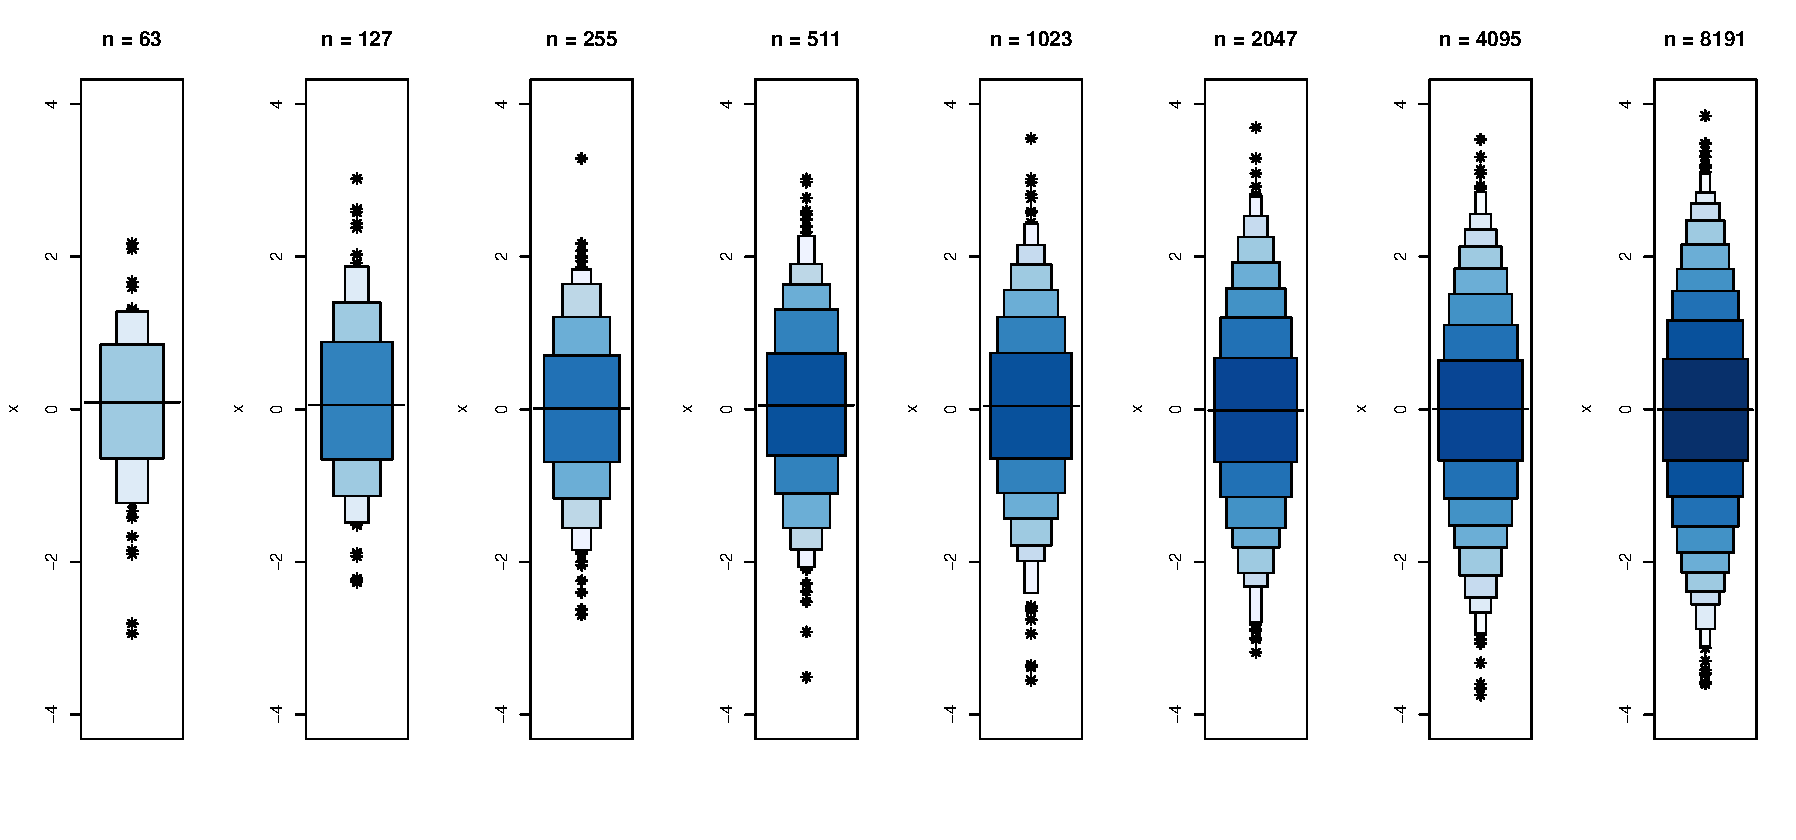
\includegraphics[width=6in]{boxplot-series.pdf}
\caption{\it \label{series} Series of 8 letter value box plots showing normally distributed random samples. From left to right sample sizes doubles in each plot from $2^6-1 = 63$ to $2^{13}-1=8191$.}
\end{center}
\end{figure*}

Figure \ref{biotin} shows letter value box plots of raw gene 
expression values from eight chips in a  microrarray experiment. 
Every second plot gives the values from a biological replicate 
of the previous plot.  
One typical question that has yet to be addressed
these kinds of studies is whether the expression 
levels can be compared across chips; i.e., whether 
using means or gene profiles will valid inferences from the experiment.   
The letter value box plots in figure \ref{biotin} help to compare the 
distributions between chips. In this case, it might be necessary 
to look more closely at the third and fourth chips, 
$B T_1$ and $B T_2$, as their distributions seem to be 
quite different from the other six replicates.

\begin{figure*}[hbt]
\begin{center}
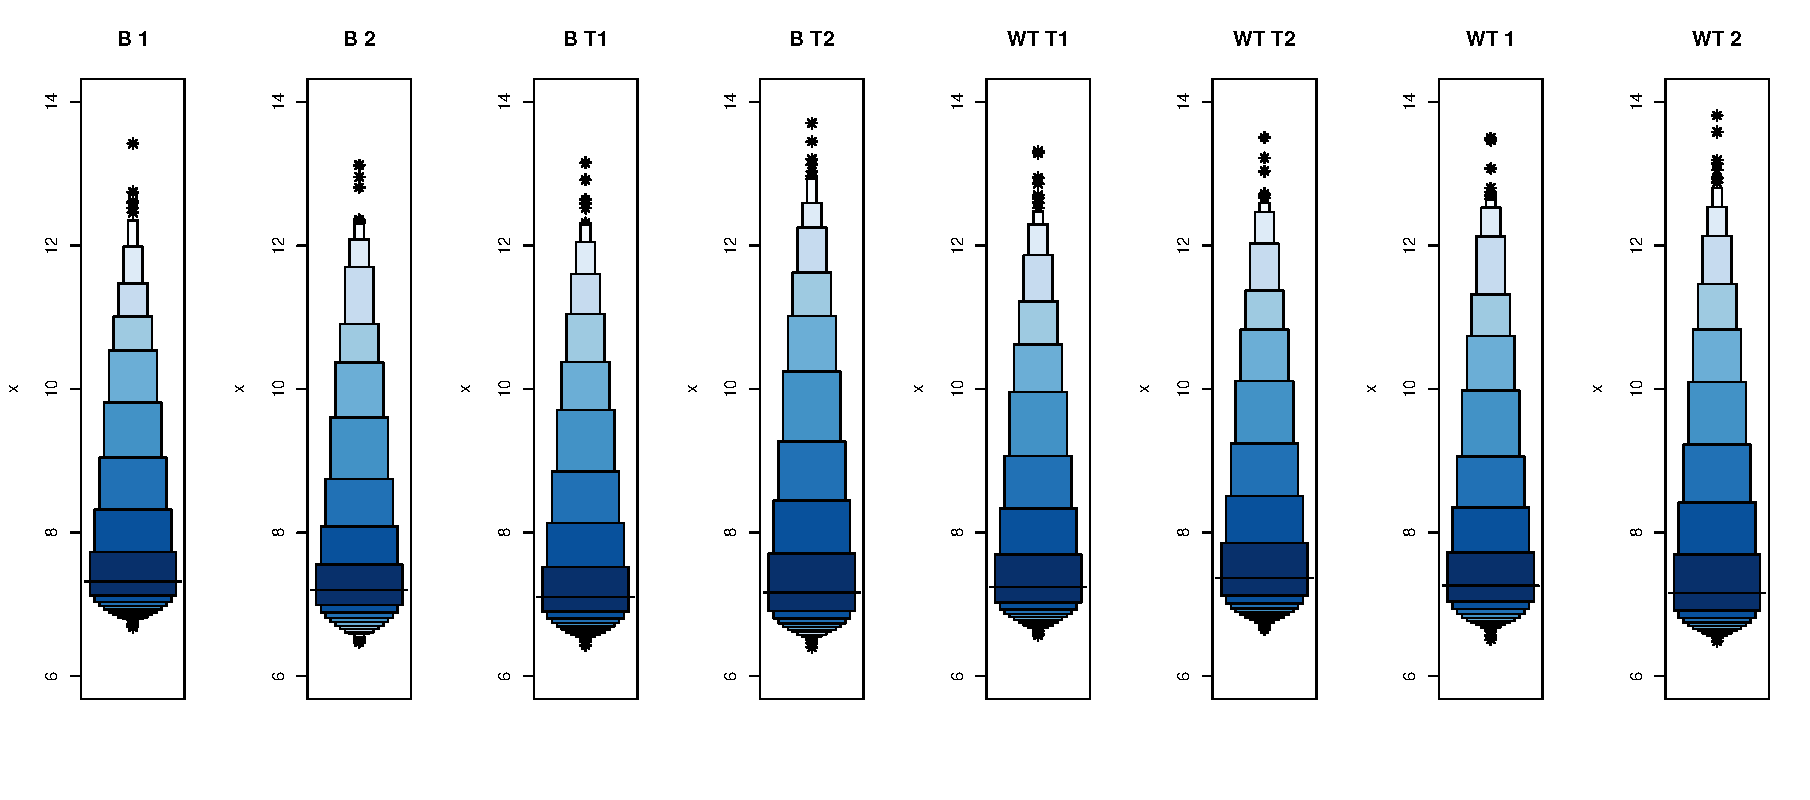
\includegraphics[width=6in]{biotin.pdf}
\caption{\it \label{biotin} Letter-value box plots of gene expressions from a microarray experiment. Raw values from eight chips are displayed side by side.}
\end{center}
\end{figure*}

\subsection*{Implementation}

The Appendix contains the R code for implementing these
letter value boxplots.  The code has been posted also on
\texttt{http://statlib.cmu.edu}.
Further information about the code and its implementation
are available from the first author.

{\tt
\begin{verbatim}
LVboxplot <- function(x, k=NULL, 
  perc=NULL, alpha=0.95, horizontal=T, 
  col=T,...) 
\end{verbatim}}

Arguments

\begin{tabular}{lp{2.5in}}
\tt x & vector of data values to be displayed \\
\tt k & number of letter-value statistics shown. \\
\tt perc & percentage of data points to be shown individually 
(as outliers) outside the letter-value boxes. {\tt perc} is only used, 
if {\tt k} is not specified.\\
\tt alpha & significance level, if neither {\tt k} 
nor {\tt perc} is specified, {\tt alpha} is used to determine how 
many letter values are to be used. 
If used, confidence intervals around each letter value statistics 
will not include neighboring letter value statistics at a 
significance level of {\tt alpha}. 
\end{tabular}

Value

\begin{tabular}{lp{2.2in}}
\tt letter.val & matrix of values (lower and upper) of all {\tt k} 
letter value statistics, including depth of each.\\
\tt conf.int & $2k-1 \times 2$ matrix of confidence intervals for 
all letter value statistics using the significance value as 
specified in {\tt alpha}.\\ 
\tt outliers & list of all individually drawn points (outliers 
in a standard box plot).\\
\end{tabular}

\bibliographystyle{asa}
\bibliography{references}
\end{document} 
